\documentclass[11pt,a4paper,titlepage,draft]{article}
\usepackage[utf8]{inputenc}
\usepackage[greek]{babel}
\usepackage{amsmath}
\usepackage{amsfonts}
\usepackage{amssymb}
\usepackage{commath}
\usepackage{xcolor}
\usepackage{hyperref}
\usepackage[skins,theorems]{tcolorbox}
\usepackage{titlesec}

\usetikzlibrary{arrows.meta}

\usepackage[left=2cm,right=2cm,top=2cm,bottom=2cm]{geometry}

\makeatletter
%\newcommand{\attnboxed}[1]{\textcolor{red}{\fbox{\normalcolor\m@th$\displaystyle#1$}}}
\makeatother
\tcbset{highlight math style={enhanced,colframe=red,colback=white,%
  arc=0pt,boxrule=1pt,shrink tight,boxsep=1.5mm,extrude by=0.5mm}}
\newcommand{\attnboxed}[1]{\tcbhighmath[colback=red!5!white,drop fuzzy shadow,arc=0mm]{#1}}
\titleformat{\section}{\bf\Large}{Κεφάλαιο \thesection}{1em}{}
\newtcolorbox{attnbox}[1]{colback=red!5!white,%
  colframe=red!75!black,fonttitle=\bfseries,title=#1}
\newtcolorbox{infobox}[1]{colback=blue!5!white,%
  colframe=blue!75!black,fonttitle=\bfseries,title=#1}


\title{Σημειώσεις Στατιστική \& Πιθανότητες}
\date{2016, Εαρινό εξάμηνο}
\author{Καναβούρας Κωνσταντίνος \\ \textlatin{\url{http://users.auth.gr/konkanant}}}



\begin{document}

\maketitle

%\tableofcontents

\newpage

\begin{itemize}
\item Γ. Ζιούτας Πιθανότητες
\item Δ. Κουγιουμτζής Στατιστική
\item Βιβλίο: Πιθανότητες και Στατιστική για Μηχανικούς, Γ. Ζιούτας
\end{itemize}

\paragraph{}

\begin{itemize}
\item Εξετάσεις: 8 μονάδες (τουλάχιστον 4/8 για να περάσει)
\item \textlatin{Test}: 2 μονάδες
\end{itemize}

\part{Πιθανότητες}

\section{}
\paragraph{Είδη φαινομένων}

\begin{enumerate}
\item \textbf{Αιτιοκρατικά} (καθοριστικά): Ξέρω το αποτέλεσμα του φαινομένου όταν γνωρίζω τα αίτια/τις προϋποθέσεις/το περιβάλλον του.
\item \textbf{Στοχαστικά}: Δεν μπορώ να προβλέψω το αποτέλεσμα, ακόμα και αν γνωρίζω τα παραπάνω.
\end{enumerate}
Μπορεί να υπάρχει και αβεβαιότητα λόγω μη ιδανικών μοντέλων πρόβλεψης. Ο μηχανικός πρέπει να γνωρίζει και να μπορεί να μετρά αυτήν την αβεβαιότητα.

\subsection{Πείραμα τύχης}
Στοχαστικό φαινόμενο που μπορούμε να δοκιμάσουμε όσες φορές θέλουμε, ακριβώς με τις ίδιες συνθήκες, και γνωρίζουμε όλα τα δυνατά αποτελέσματα, αν και δε γνωρίζουμε ακριβώς το αποτέλεσμα κάθε πειράματος.

\begin{itemize}
\item \(E\): Πείραμα τύχης (\textlatin{Experiment})
\item \(S\): \( \left\lbrace s_1,s_2, \dots , s_n \right\rbrace\) Δειγματοχώρος (\textlatin{Sample space})
\item \(s_i\): Δειγματοσημεία
\end{itemize}

\textit{π.χ.}
\begin{align*}
E_1 \qquad & S_1 = \left\lbrace 1,2,3,4,5,6 \right\rbrace \rightarrow \text{ ρίψη ζαριού}\\
E_2 \qquad & S_2 = \left\lbrace KKK, KK\Gamma , K\Gamma K, \Gamma K K, K \Gamma \Gamma, \Gamma \Gamma K, \Gamma \Gamma \Gamma \right\rbrace \rightarrow \text{ ρίψη κέρματος 3 φορές} \\
E_3 \qquad & S_3 = \left\lbrace 0,1,\dots,N \right\rbrace \rightarrow \text{ ελαττωματικά προϊόντα}\\
E_4 \qquad & S_4 = \left\lbrace 0,1,2,3\dots \right\rbrace \rightarrow \text{ αριθμός ατόμων που εκπέμπει ραδιενεργό υλικό}\\
E_5 \qquad & S_5 = \left\lbrace x | x \geq 0, x \in \mathbb R \right\rbrace \rightarrow \text{ χρόνος γενονότος}
\end{align*}

\paragraph{}
Υποσύνολα του δειγματικού χώρου, π.χ. \(A = \left\lbrace 4,5,6 \right\rbrace \subseteq S\) ονομάζονται γεγονότα. Συνήθως συμβολίζονται \(A,B,W,R\). Λέμε ότι ένα γεγονός πραγματοποιείται.

Το \(S\) είναι σίγουρο γεγονός.

το \(\left\lbrace \right\rbrace \subseteq S \) ονομάζεται αδύνατο γεγονός και συμβολίζεται \( \emptyset \).

\paragraph{}
\[S =  \left\lbrace s_1,s_2,\dots,s_n  \right\rbrace \]

Το δυναμοσύνολο \(S^*\) περιέχει όλα τα δυνατά υποσύνολα του \(S\):
\[S^* =  \left\lbrace  \left\lbrace  \right\rbrace,  \left\lbrace s_1 \right\rbrace, \left\lbrace s_2 \right\rbrace, \dots,  \left\lbrace s_n  \right\rbrace,  \left\lbrace s_1,s_2 \right\rbrace, \left\lbrace s_1,s_3 \right\rbrace, \dots,  \left\lbrace s_1,s_2,s_3 \right\rbrace \dots  \right\rbrace \]

Είναι:
\begin{align*}
(a+b)^n &= \binom{n}{0}a^nb^0 + \binom{n}{1}a^{n-1}b^1 + \binom{n}{2}a^{n-2}b^2 + \dots + \binom{n}{n} a^0b^n \\
(1+1)^n &= \binom{n}{0}\cdot 1 + \binom{n}{1}\cdot 1 + \binom{n}{2} \cdot 1+ \dots + \binom{n}{n} \cdot 1 \\
2^n &= \binom{n}{0} + \binom{n}{1} + \binom{n}{2} + \dots + \binom{n}{n}
\end{align*}
Παρατηρούμε ότι το \(S^*\) έχει \(2^n\) στοιχεία αν το \(S\) έχει \(n\).

\section*{Διαγράμματα \textlatin{Venn}}

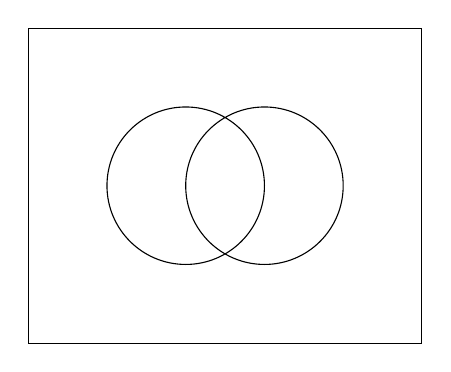
\begin{tikzpicture}[fill=gray]
% left hand
\scope
\clip (-2,-2) rectangle (2,2)
      (1,0) circle (1);
\endscope
% right hand
\scope
\clip (-2,-2) rectangle (2,2)
      (0,0) circle (1);
\endscope
% outline
\draw (0,0) circle (1)
      (1,0) circle (1);
\draw (-2,-2) rectangle (3,2);
\end{tikzpicture}

\paragraph{Ισότητα}
\begin{tikzpicture}[fill=gray]
\draw (0,0) circle (1) node[above] {$A$} node[below] {$B$};
\draw (-2,-2) rectangle (3,2) node[anchor=west] {$S$};
\end{tikzpicture}

\paragraph{Περιεκτικότητα}
\begin{tikzpicture}[fill=gray]
\draw (0,0) circle (1) node[above] {$A$};
\draw (-0.5,-0.5) circle (0.3) node[above] {$B$};
\draw (-2,-2) rectangle (3,2) node[anchor=west] {$S$};
\end{tikzpicture}

\paragraph{Συμπλήρωμα}
\paragraph{Ισότητα}
\begin{tikzpicture}[fill=gray]
\draw (0,0) circle (1) node[above] {$A$} node[below] {$\overline{A}$};
\draw (-2,-2) rectangle (3,2) node[anchor=west] {$S$};
\end{tikzpicture}

\subsubsection{Πράξεις}
\paragraph{Ένωση \(A \cup B\)}
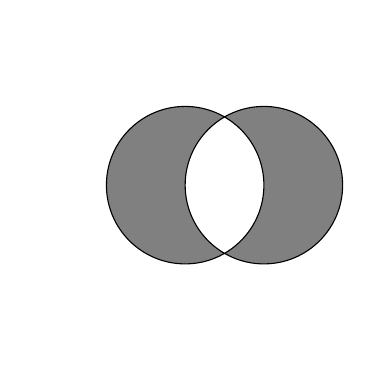
\begin{tikzpicture}[fill=gray]
% left hand
\scope
\clip (-2,-2) rectangle (2,2)
      (1,0) circle (1);
\fill (0,0) circle (1);
\endscope
% right hand
\scope
\clip (-2,-2) rectangle (2,2)
      (0,0) circle (1);
\fill (1,0) circle (1);
\endscope
% outline
\draw (0,0) circle (1)
      (1,0) circle (1);
\end{tikzpicture}

\paragraph{Τομή \(A \cap B\)}
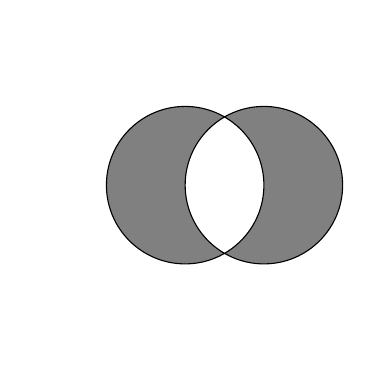
\begin{tikzpicture}[fill=gray]
% left hand
\scope
\clip (-2,-2) rectangle (2,2)
      (1,0) circle (1);
\fill (0,0) circle (1);
\endscope
% right hand
\scope
\clip (-2,-2) rectangle (2,2)
      (0,0) circle (1);
\fill (1,0) circle (1);
\endscope
% outline
\draw (0,0) circle (1)
      (1,0) circle (1);
\end{tikzpicture}

\paragraph{Διαφορά \(A - B\)}
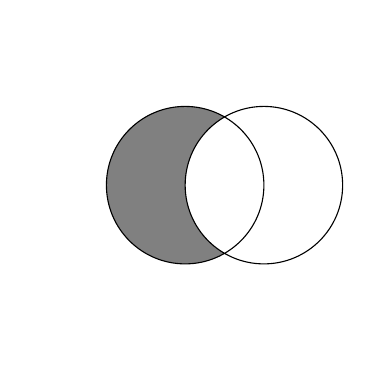
\begin{tikzpicture}[fill=gray]
% left hand
\scope
\clip (-2,-2) rectangle (2,2)
      (1,0) circle (1);
\fill (0,0) circle (1);
\endscope
% right hand
\scope
\clip (-2,-2) rectangle (2,2)
      (0,0) circle (1);
%\fill (1,0) circle (1);
\endscope
% outline
\draw (0,0) circle (1)
      (1,0) circle (1);
\end{tikzpicture}
Παρατηρώ ότι:
\begin{align*}
(x-y)+y &= x \\
(A-B) \cup B &= A \cup B
\end{align*}

\subsubsection{Ιδιότητες}
\begin{itemize}
\item \(A \cup B = B \cup A\)
\item \(A \cup \left( B \cup \Gamma \right) = \left( A \cup B \right) \Gamma \)
\item \(A \cup \left( B \cap \Gamma \right) = \left( A \cup B \right) \cap \left( A \cup \Gamma \right) \)
\item \( \overline{A \cup B} = \overline{A} \cap \overline{B} \)
\end{itemize}

\subsubsection{}
\begin{align*}
S &=  \left\lbrace KK, K\Gamma, \Gamma K, \Gamma \Gamma \right\rbrace \\
A &=  \left\lbrace KK, K \Gamma, \Gamma K  \right\rbrace \leftarrow \text{ τουλάχιστον μία κεφαλή} \\
B &= \left\lbrace KK, \Gamma K  \right\rbrace \leftarrow \text{ κεφαλή στη 2η ρίψη} \\
\end{align*}
\begin{align*}
A\cup B &=  \left\lbrace KK, K \Gamma , \Gamma K  \right\rbrace \\
A\cap B &=  \left\lbrace KK,  \Gamma K  \right\rbrace \\
A-B &=  \left\lbrace K \Gamma  \right\rbrace
\end{align*}

\subsubsection{}
\[S,A,B, \Gamma \]
\begin{itemize}
\item Τουλάχιστον ένα από \(A,B, \Gamma \): \(A \cup B \cup  \Gamma \)
\item Μόνο ένα από τα \(Α,Β, \Gamma \): \(
\left( A - \left( B \cup \Gamma \right) \right) \cup
\left( B - \left( A \cup \Gamma \right) \right) \cup
\left( \Gamma  - \left( A \cup B \right) \right) =
\left( A \cap \overline{B} \cap \overline{C} \right) \cap
\left( \overline{A} \cap B \cap \overline{C} \right) \cap
\left( \overline{A} \cap \overline{B} \cap C \right)
\)
\item Ακριβώς δύο από τα \(A,B \Gamma \):
\(
\left(A \cap B - \Gamma \right) \cap
\left(A \cap \Gamma  - B \right) \cap
\left(B \cap  \Gamma - A \right)
\)
\item Το πολύ δύο από τα \(A,B, \Gamma\):
\(
\overline{A \cap B \cap \Gamma } = \overline{A} \cup \overline{B} \cup \overline{C}
\)
\end{itemize}

\paragraph{}
\textit{π.χ.}
\[A,B, \Gamma \]
Σε ένα παιχνίδι όπου κερδίζει ο παίκτης που πρώτος φέρνει κεφαλή, ποιο είναι το γεγονός να κερδίσει ο \(A\), αν \(A_i, B_i, \Gamma_i\) τα ενδεχόμενα στην \(i\)-οστή ρίψη να κερδίσει ένας παίκτης.
\[
WA = A_1 \cup \left( \overline{A_1} \cap \overline{B_2} \cap \overline{\Gamma_3} \cap A_4 \right) \cup \left( \overline{A_4} \cap \overline{B_5} \cap \overline{\Gamma_6} \cap A_7 \right) \cup \dots
\]

Να βρεθούν τα \(WB, W \Gamma \).
\end{document}